\section{\K 信号处理}
\subsection{\K 电压比较器}
\Par 电压比较器工作在饱和区,因此它只满足虚断原则,不满足虚短原则.如图\ref{fig:单限电压比较器}所示,它是一个单限电压比较器,根据理想集成运算放大器的特性,当$U_R>u_i$时,它工作在正饱和区,输出电压为正;当$U_R<u_i$时,它工作在负饱和区,输出电压为负.由此,实现了输入电压$u_i$与$U_R$的比较.
\begin{figure}[htbp]
	\centering
	\begin{minipage}[b]{0.48\textwidth}
        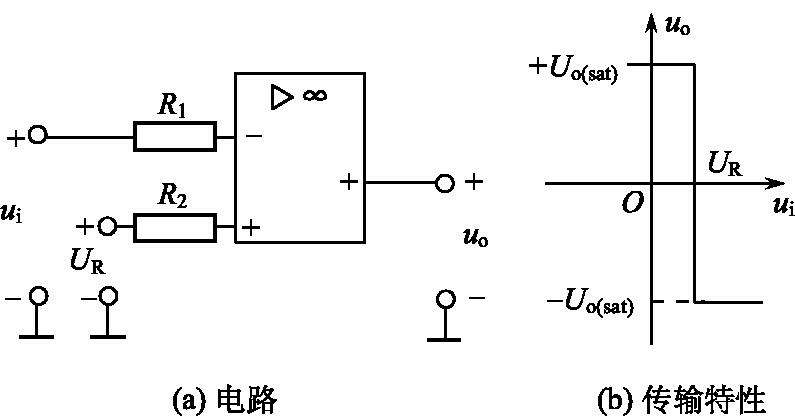
\includegraphics[width=0.85\textwidth]{单限电压比较器.jpg}
	    \caption{单限电压比较器}
	    \label{fig:单限电压比较器}
    \end{minipage}
    \begin{minipage}[b]{0.48\textwidth}
        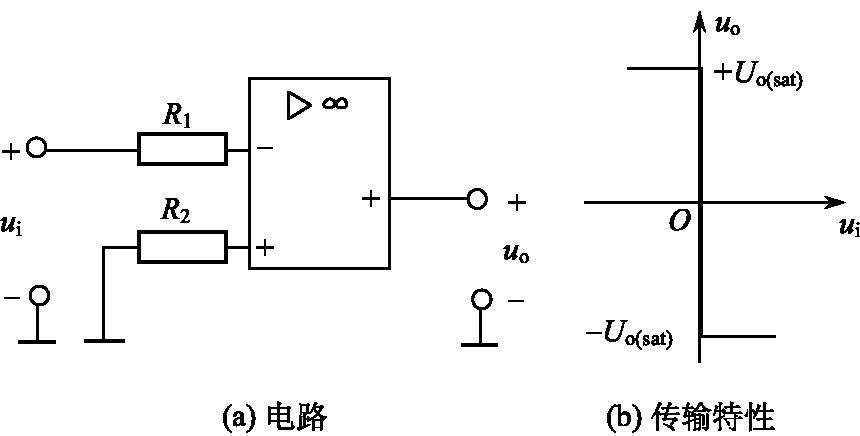
\includegraphics[width=0.85\textwidth]{过零比较器.jpg}
	    \caption{过零比较器}
	    \label{fig:过零比较器}
    \end{minipage}
\end{figure}

\Par 当$U_R=0$,即输入端正相极接地时,它便构成了过零比较器.同时,由于输出的电压常常过大,我们便加上了双向稳压二极管,如图\ref{fig:限幅电压比较器传输特性}所示,当$U_R>u_i$时,输出的电压为正,此时双向稳压二极管上端导通,下端稳压,使得输出电压维持在稳压电压$U_Z$.$U_R>u_i$的情况同理可得,输出电压是反向的稳压电压$U_Z$.

\begin{figure}[htbp]
	\centering
	\begin{minipage}[b]{0.48\textwidth}
        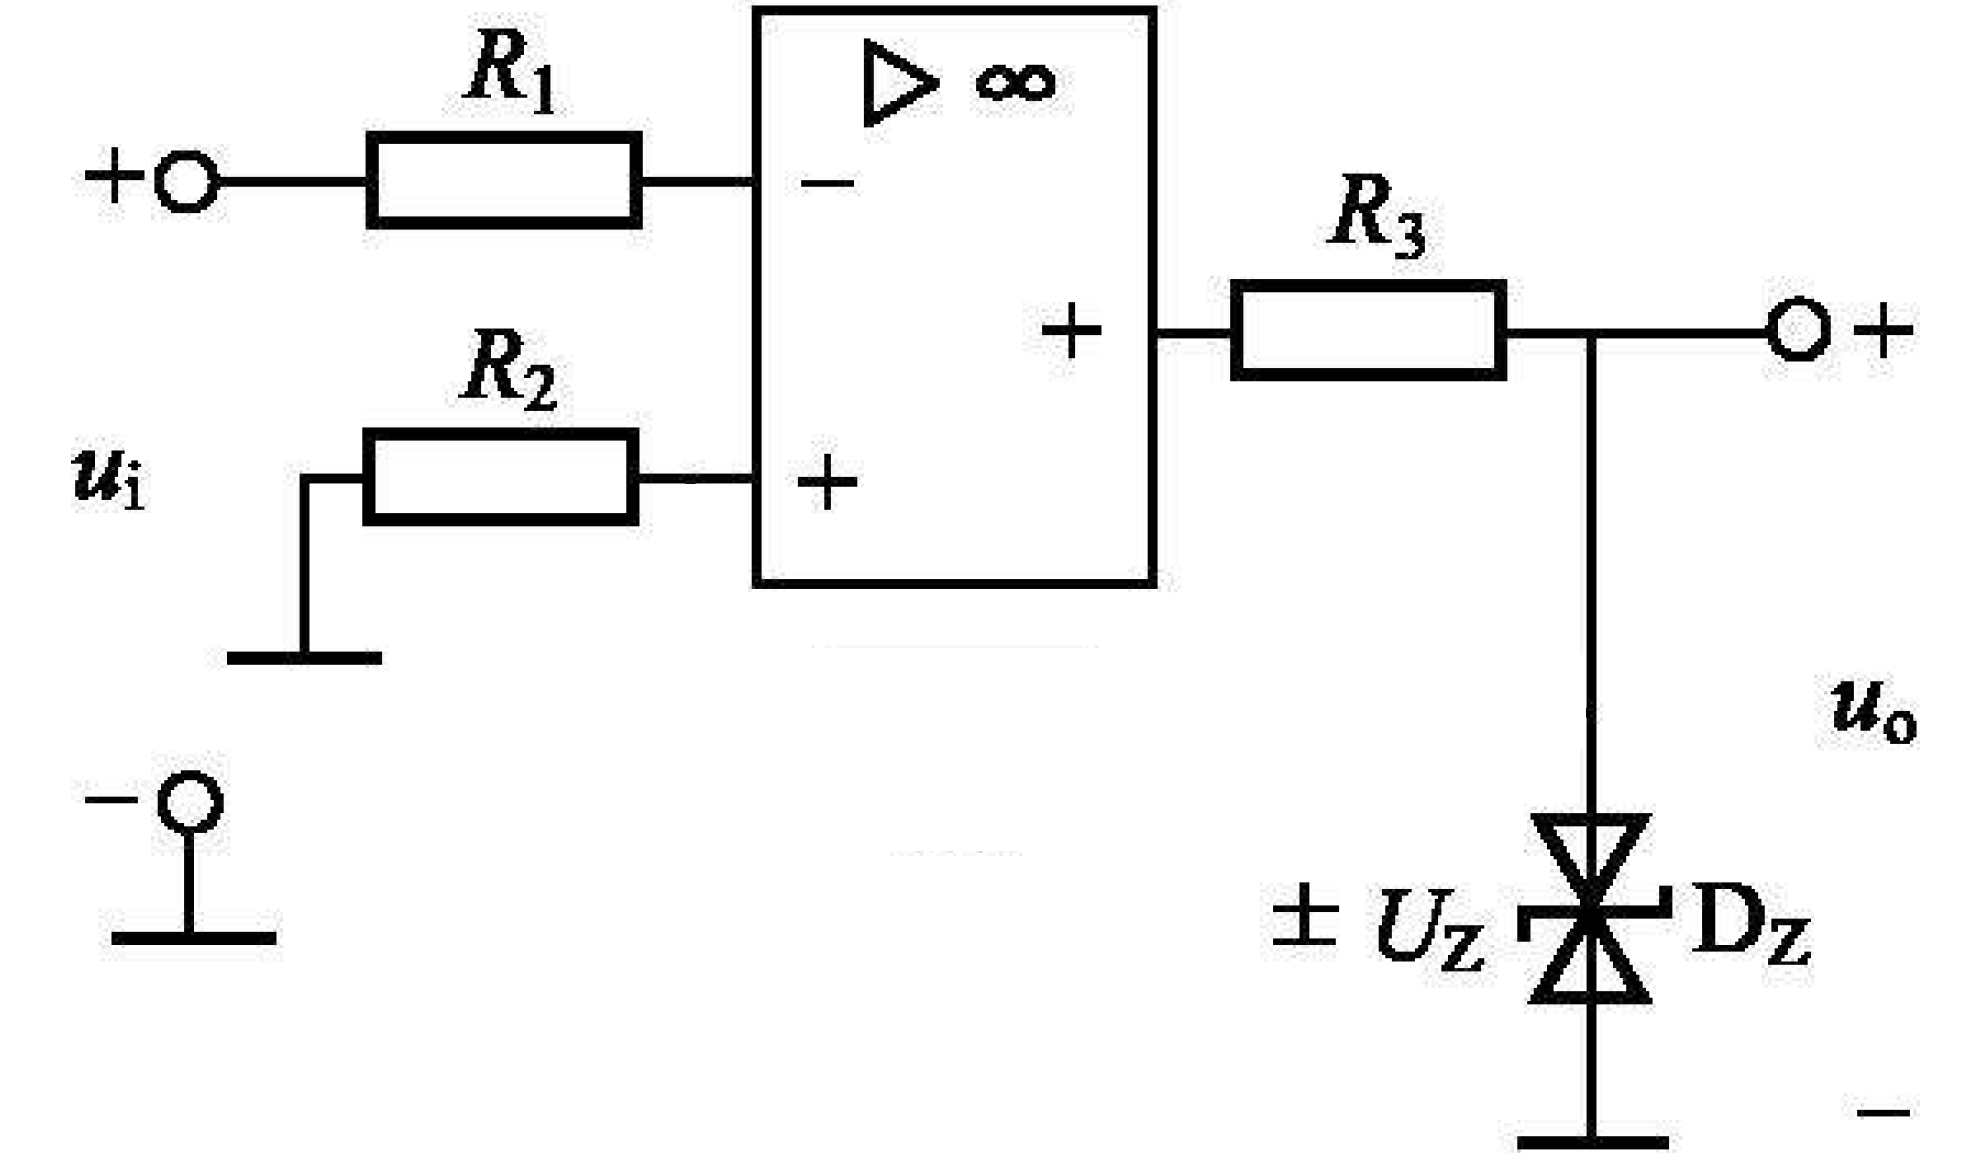
\includegraphics[width=0.85\textwidth]{限幅电压比较器电路.png}
	    \caption{电路}
	    \label{fig:限幅电压比较器电路}
    \end{minipage}
    \begin{minipage}[b]{0.48\textwidth}
        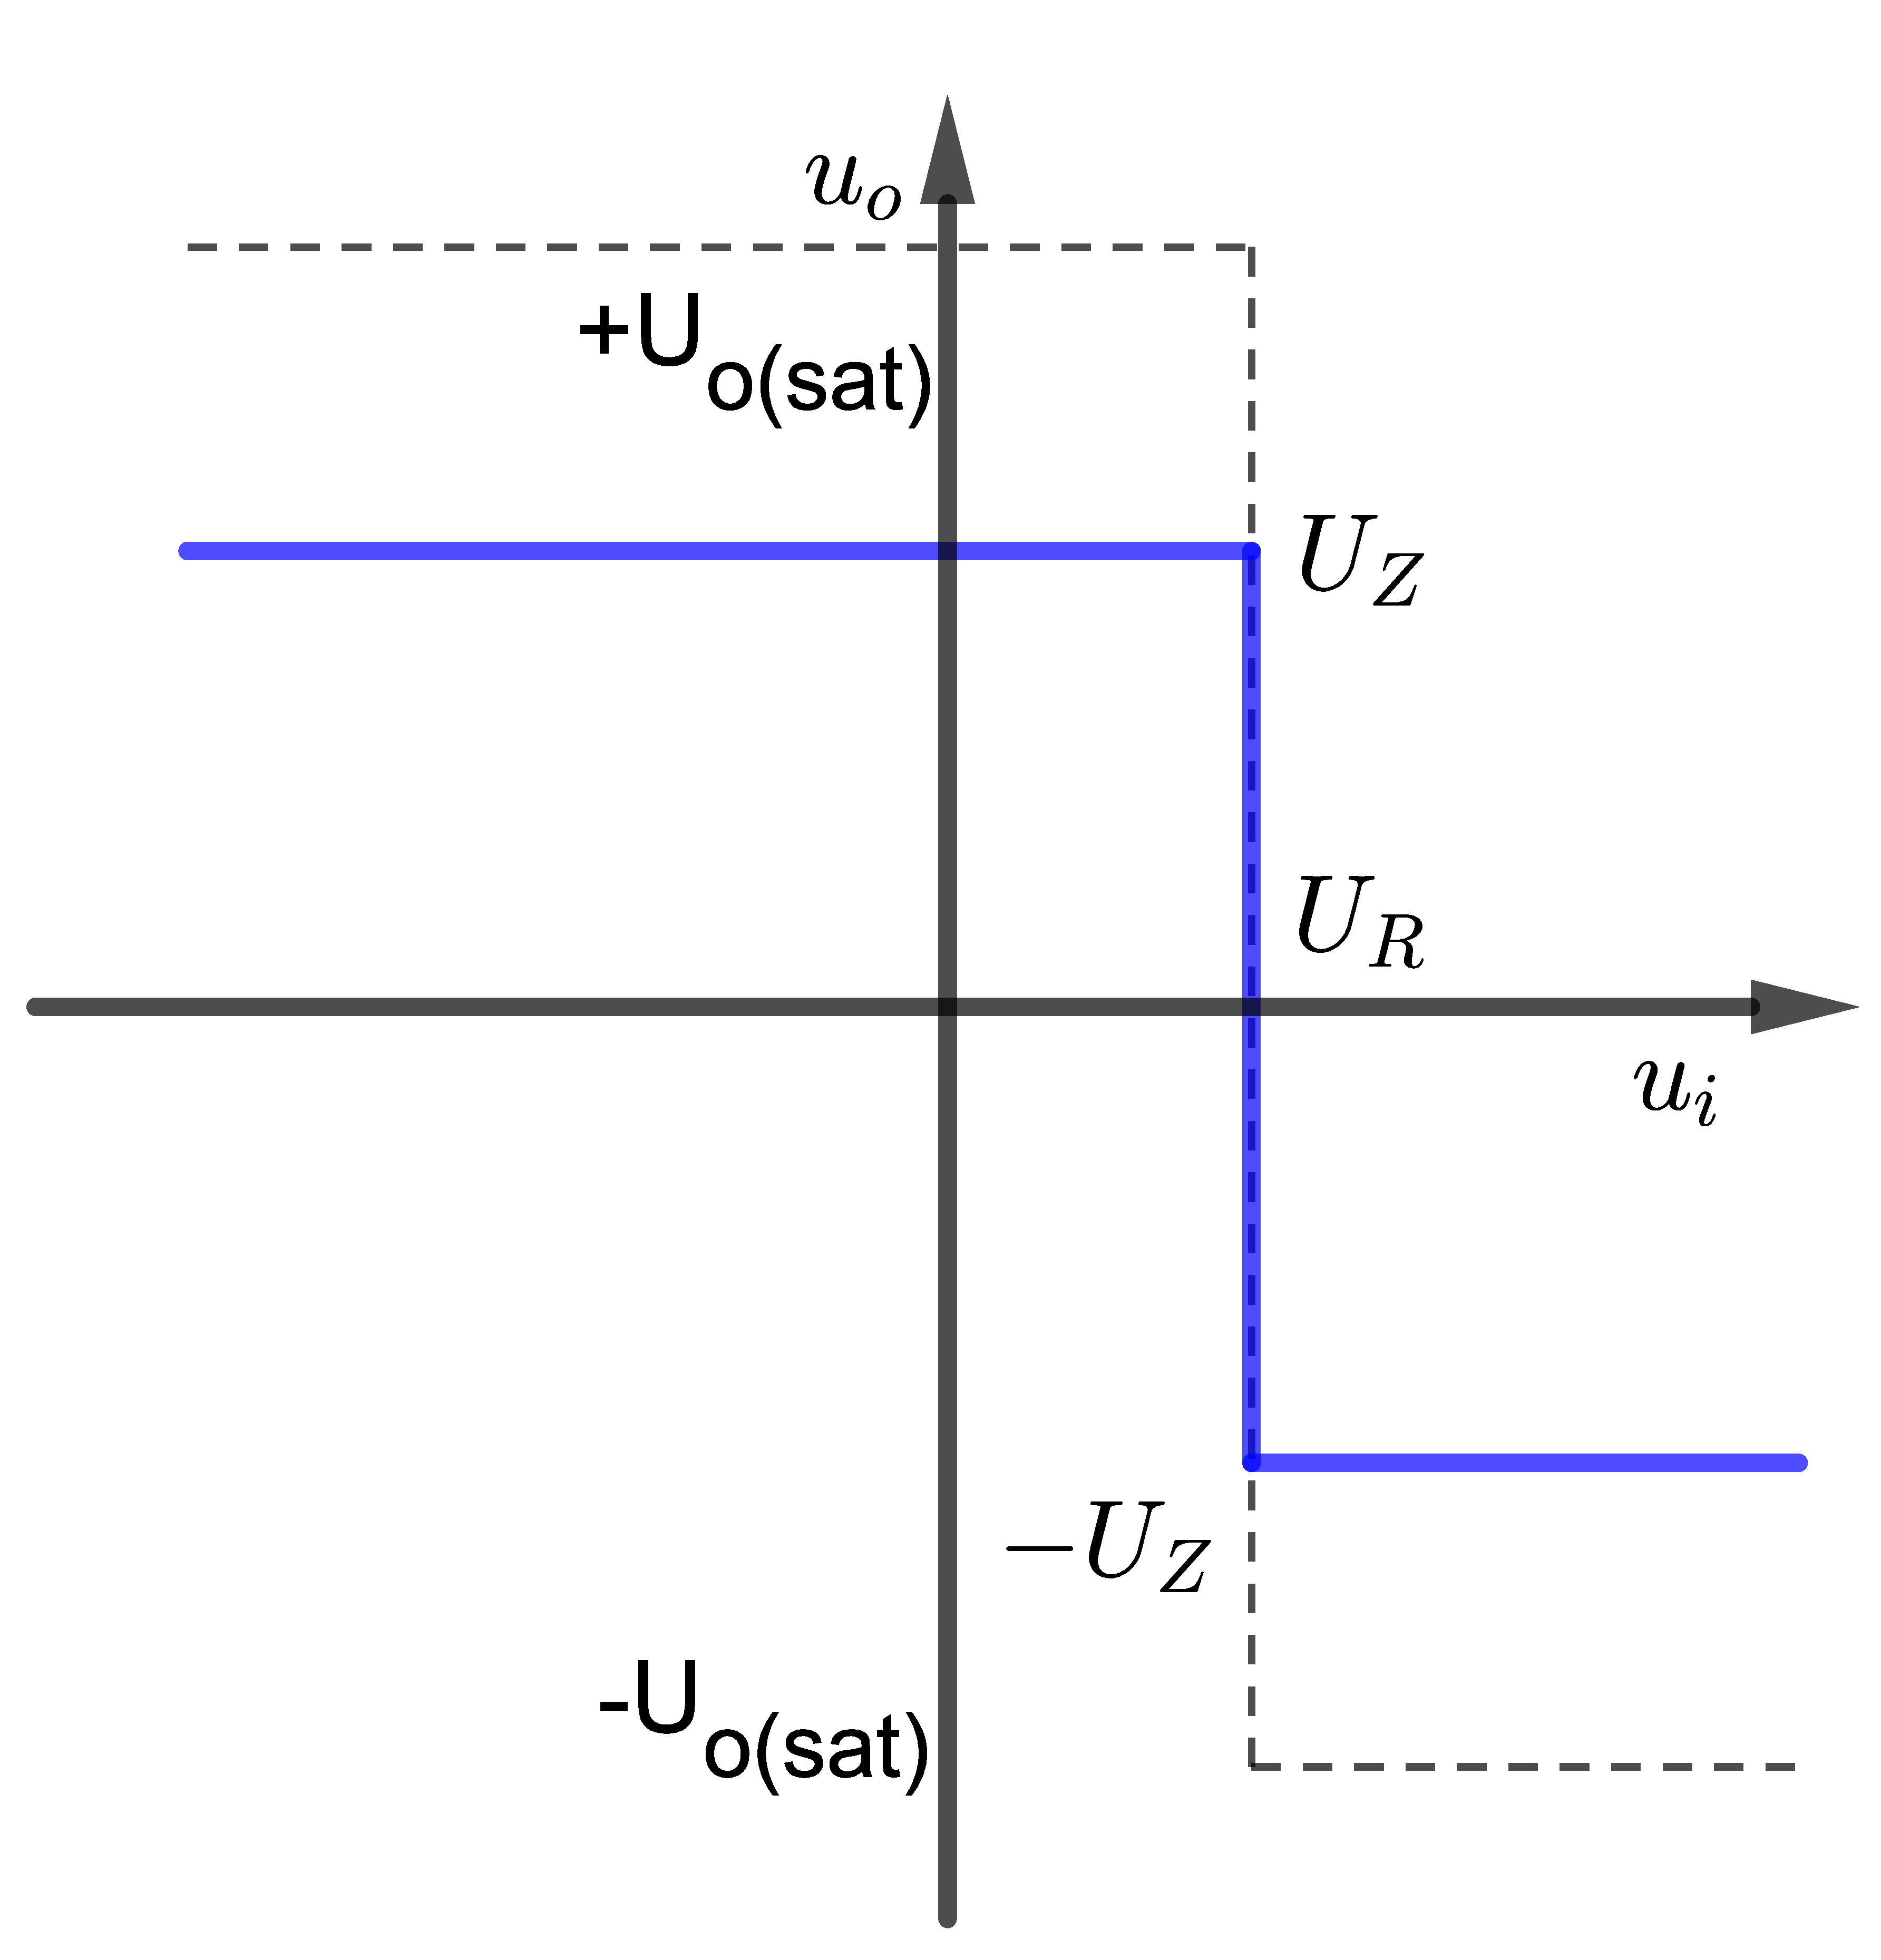
\includegraphics[width=0.65\textwidth]{限幅电压比较器传输特性.pdf}
	    \caption{传输特性}
	    \label{fig:限幅电压比较器传输特性}
    \end{minipage}
\end{figure}
\Par 通过电压比较器,我们很容易就可以将正弦电压转化成方波电压.
